\chapter{Testing Framework}

	This section describes a typical testing framework that can be developed within an organization. 
	It can be seen as a reference framework that comprises techniques and tasks that are appropriate 
	at various phases of the software development life cycle (SDLC).

	There are many development methodologies such as the Rational Unified Process, eXtreme and Agile 
	development, and traditional waterfall methodologies. The intent of this guide is to suggest
	neither a particular development methodology nor provide specific guidance that adheres to any 
	particular methodology. Instead, we are presenting a generic development model, and the reader 
	should follow it according to their company process.
	
	This testing framework consists of the following activities that should take place:
		\begin{itemize}
			\item Before Development Begins
			\item During Definition and Design
			\item During Development
			\item During Deployment
			\item Maintenance and Operations
		\end{itemize}

	\clearpage
	\section{Before Development Begins}
		Before application development has started:
		
		{\bf Review Policies and Standards} \\
			Ensure that there are appropriate policies, standards, and documentation in place. 
			Documentation is extremely important as it gives development teams guidelines and 
			policies that they can follow. People can only do the right thing, if they know what 
			the right thing is.

		{\bf Develop Measurement and Metrics Critera} \\
			Before development begins, plan the measurement program. By defining criteria that 
			need to be measured, it provides visibility into defects in both the process and product. 
			It is essential to define the metrics before development begins, as there may be a need 
			to modify the process in order to capture the data.

	\section{During Definition and Design}

		{\bf Review Security Requirements} \\
			Security requirements define how an application works from a security perspective. It is essential 
			that the security requirements be tested. Testing in this case means testing the assumptions 
			that are made in the requirements, and testing to see if there are gaps in the requirements 
			definitions. When looking for requirements gaps, consider looking at security mechanisms such as:
			User Management (password reset etc.), Authentication, Authorization, Data Confidentiality, 
			Integrity, Accountability, Session Management, Transport Security, Tiered System Segregation
			and Privacy.

		{\bf Review Design and Architecture} \\
			Applications should have a documented design and architecture. By documented, we mean 
			models, textual documents, and other similar artifacts. It is essential to test these 
			artifacts to ensure that the design and architecture enforce the appropriate level of 
			security as defined in the requirements. Identifying security flaws in the design phase 
			is not only one of the most cost-efficient places to identify flaws, but can be one of 
			the most effective places to make changes.

		{\bf Create And Review UML Models} \\
			Once the design and architecture is complete, build Unified Modeling Language (UML) 
			models that describe how the application works. In some cases, these may already be 
			available. Use these models to confirm with the systems designers an exact understanding 
			of how the application works. If weaknesses are discovered, they should be given to 
			the system architect for alternative approaches.

		{\bf Create And Review Threat Models} \\
			Armed with design and architecture reviews, and the UML models explaining exactly how 
			the system works, undertake a threat modeling exercise. Develop realistic threat 
			scenarios. Analyze the design and architecture to ensure that these threats have been 
			mitigated, accepted by the business, or assigned to a third party, such as an insurance 
			firm. When identified threats have no mitigation strategies, revisit the design and 
			architecture with the systems architect to modify the design.


	\section{During Development} 
		Theoretically, development is the implementation of a design. However, in the real world, many 
		design decisions are made during code development. These are often smaller decisions that were 
		either too detailed to be described in the design, or in other cases, issues where no policy or 
		standard guidance was offered. If the design and architecture were not adequate, the developer 
		will be faced with many decisions. If there were insufficient policies and standards, the 
		developer will be faced with even more decisions.
		
		{\bf Code Walkthroughs} \\
		The security team should perform a code walkthrough with the developers, and in some cases, the 
		system architects. A code walkthrough is a high-level walkthrough of the code where the developers 
		can explain the logic and flow of the implemented code. It allows the code review team to obtain 
		a general understanding of the code, and allows the developers to explain why certain things were 
		developed the way they were. The purpose is not to perform a code review, but to understand at a 
		high level the flow, the layout, and the structure of the code that makes up the application.
		
		{\bf Code Reviews} \\
		Armed with a good understanding of how the code is structured and why certain things were coded 
		the way they were, the tester can now examine the actual code for security defects.
		Static code reviews validate the code against a set of checklists, including:
			\begin{itemize}
				\item Business requirements for availability, confidentiality, and integrity.
				\item OWASP Guide or Top 10 Checklists for technical exposures.
				\item Specific issues relating to the language or framework in use.
				\item Any industry specific requirements, such as ISO standards, or other regulatory regimes.
			\end{itemize}


	\section{During Deployment}
		{\bf Application Penetration Testing} \\
		Having tested the requirements, analyzed the design, and performed code review, it might be 
		assumed that all issues have been caught. Hopefully, this is the case, but penetration testing 
		the application after it has been deployed provides a last check to ensure that nothing has 
		been missed.
		
		{\bf Configuration Management Testing} \\
		The application penetration test should include the checking of how the infrastructure was 
		deployed and secured. While the application may be secure, a small aspect of the configuration 
		could still be at a default install stage and vulnerable to exploitation.


	\section{Maintenance and Operations}
		{\bf Conduct Operational Management Reviews} \\
			There needs to be a process in place which details how the operational side of both the 
			application and infrastructure is managed.

		{\bf Conduct Periodic Health Checks} \\
			Monthly or quarterly health checks should be performed on both the application and 
			infrastructure to ensure no new security risks have been introduced and that the level 
			of security is still intact.

		{\bf Enusure Change Verification} \\
			After every change has been approved and tested in the QA environment and deployed into 
			the production environment, it is vital that, as part of the change management process, 
			the change is checked to ensure that the level of security hasn’t been affected by the change.

	\clearpage

	\begin{figure}[H]
		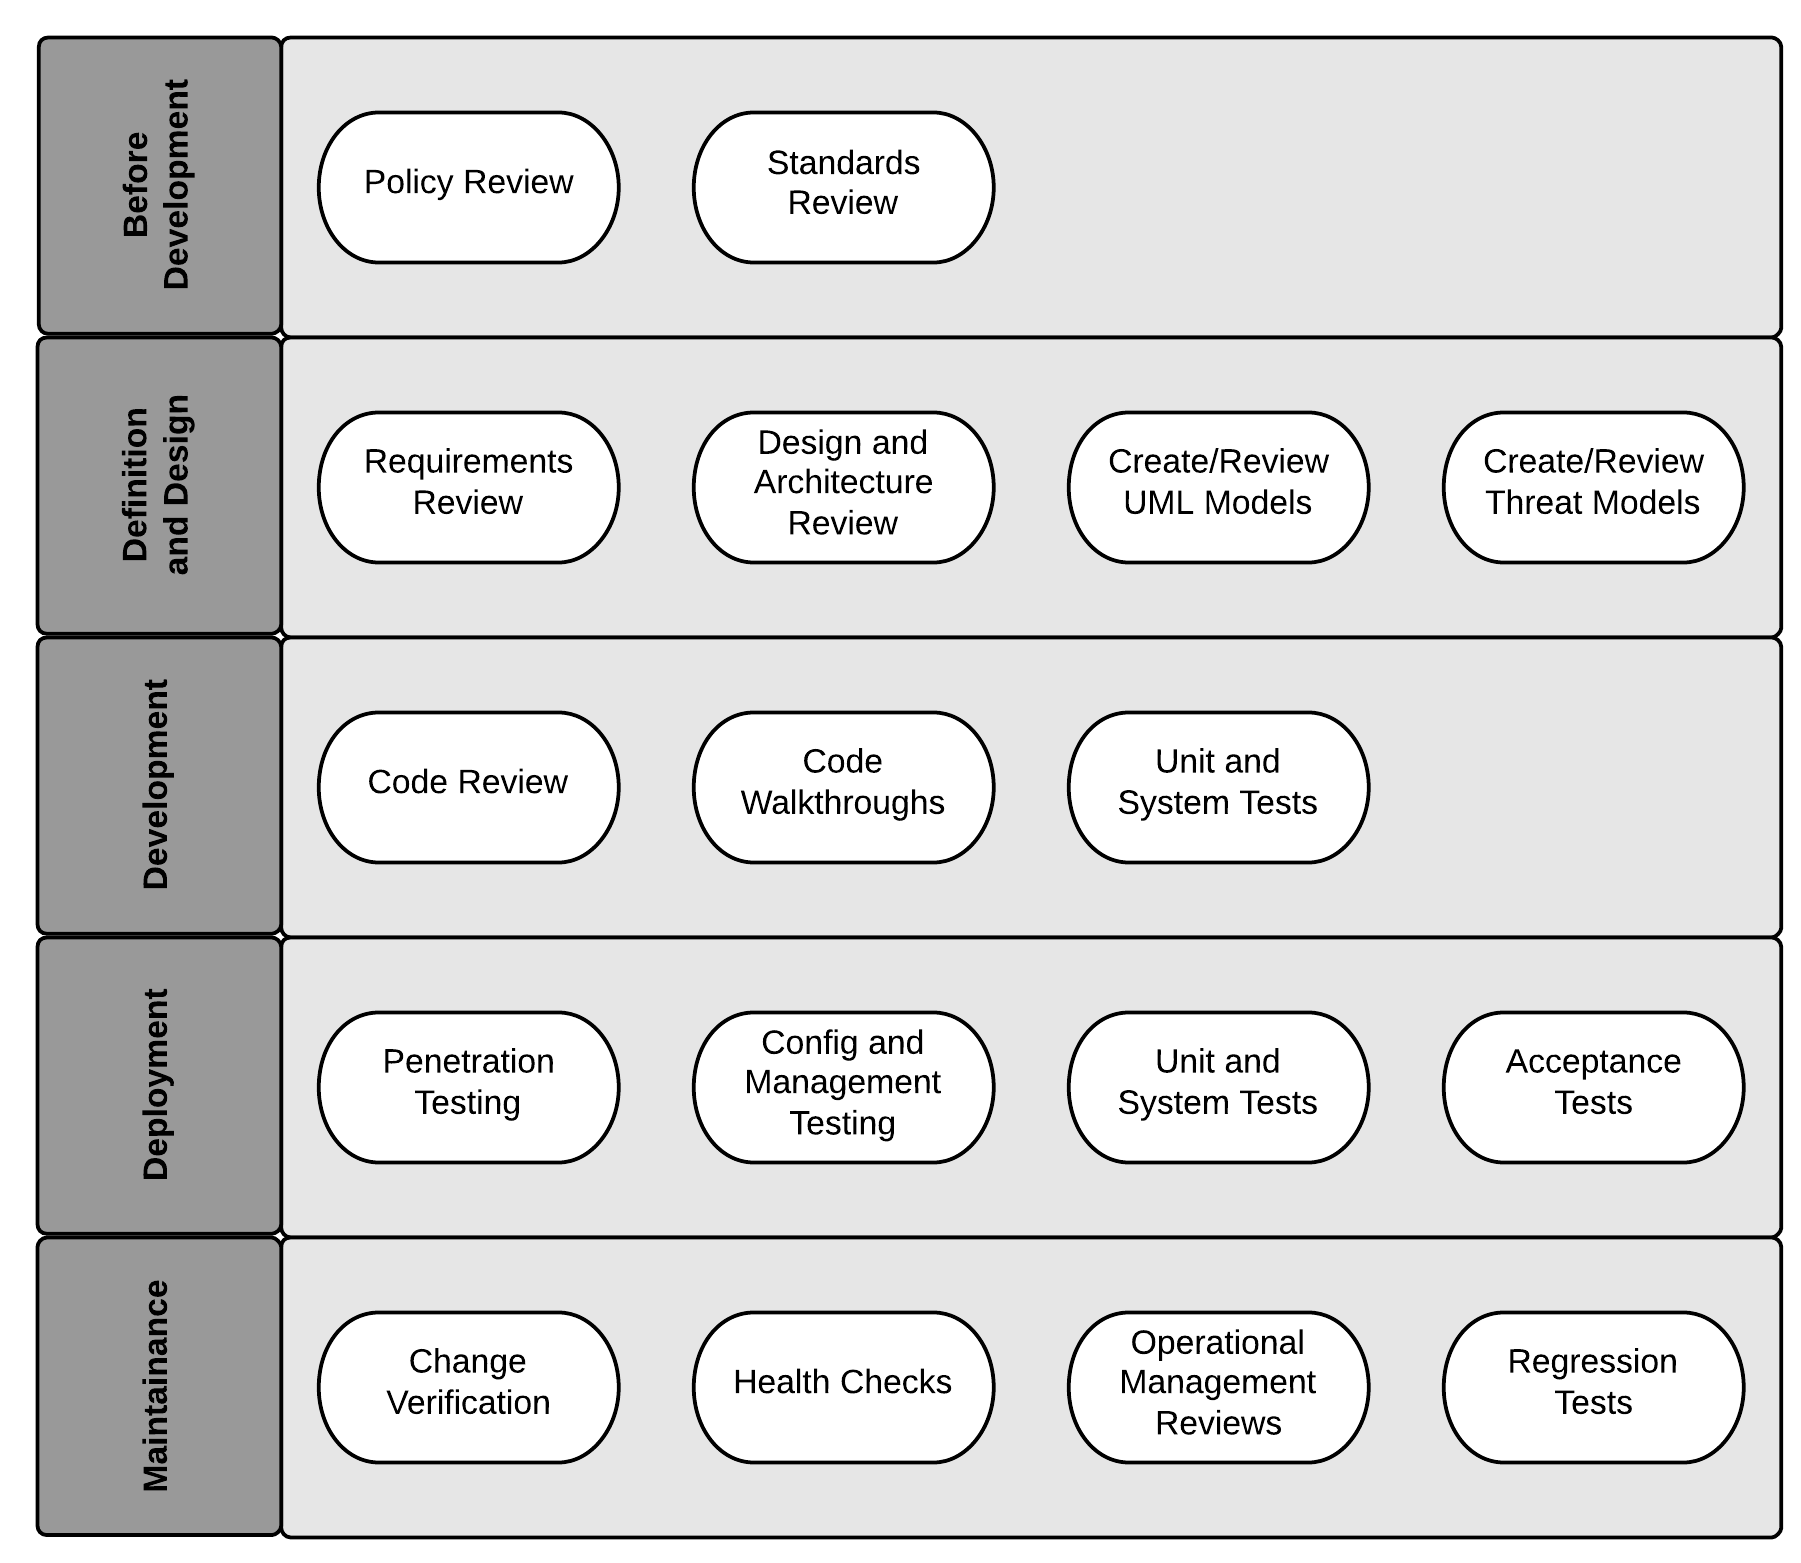
\includegraphics[width=\textwidth]{pics/testingFramework.png}
	\end{figure}

